\subsection{Structure}

\subsubsection{Block Definition Diagram}
The system consist of three parts, a random generator, an user interface and the particle swarm logic. on Figure \ref{fig:bdd} the block definition diagram can be seen with these three parts, as part of the overall Particle Swarm Optimization System.

\begin{figure}[!h]
	\centering
	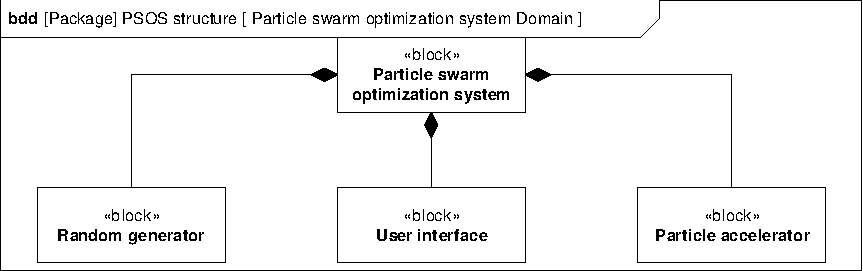
\includegraphics[width=0.8\linewidth]{diagram/bdd_particle_swarm_optimization_system.pdf}
	\caption{Block Definition Diagram of Particle Swarm Optimization System}
	\label{fig:bdd}
\end{figure}

\textbf{Random Generator:}\\
The Random Generator block is needed, to generate random seeds for use in the particle swarm algorithm.\\

\textbf{User Interface:}\\
The User Interface block needs core functionality to communicate with the system. It needs to be able to take inputs regarding the particle swarm algorithms variables and create a graphical representation of the results to the user, after a successful particle swarm analysis.\\

\textbf{Particle Accelerator:}\\
The Particle Accelerator block has the functionality to perform the particle swarm optimization algorithm. Variables for the algorithm, given by the user, are communicated via the User Interface block. The random seed for the algorithm is given by the Random Generator block.

\subsubsection{Internal Block Diagram}
Continuing with the data from the Block Definition Diagram, an Internal Block Definition Diagram (ibd) is created. Showing connections and dataflows with the ibd as seen on Figure \ref{fig:ibd}.

\begin{figure}[!h]
	\centering
	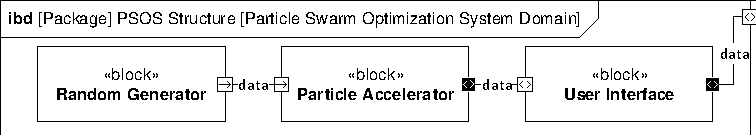
\includegraphics[width=0.8\linewidth]{diagram/ibd_particle_swarm_optimization_system.pdf}
	\caption{Internal Block Diagram of Particle Swarm Optimization System}
	\label{fig:ibd}
\end{figure}

%TODO Update ibd to include names of flowports and ports when they've been decided upon
\textbf{TODO: Update ibd to include names of flowports and ports when they've been decided upon}\\
%TODO Explain which connections are used between the blocks
\textbf{TODO: Explain which connections are used between the blocks}\\

The User uses the User Interface block, as a medium to interact with the system. The User input data to be used as variables in the particle swarm algorithm through the User Interface via a GUI. When the particle swarm algorithm has been performed by the system, the output is given to the User by the User Interface Block via a GUI.\\

The User Interface block communicates the desired variables to be used in the particle swarm algorithm to the Particle Accelerator block. When the Particle Accelerator block has performed the particle swarm algorithm, it sends the data to the User Interface block.\\

The Random Generator delivers a random seed, when needed, to the Particle Accelerator block, to be used in the particle swarm algorithm.\\

